\problemname{Pegs}

Little Zorro and Worro are playing an interesting game on an
$n\times n$ square grid. Each game is really short: each player makes just one move.
The game is played with very very thin
pegs. The pegs come in two colors: black and white. Zorro goes
first: he puts the pegs at the vertices of the grid. Then Worro
selects a subset of the pegs by drawing a convex
polygon---whatever is inside or on the boundary of the polygon is
in his set. (The pegs are so tiny that they act as points in the plane.)
For each black peg selected Worro gets \$1. For each
white peg selected Worro has to pay \$1. Naturally, Worro wants to
get as much money as possible. Now he is worried that he might not
choose the optimal set. Please, help him.

\section*{Input}
The first line contains $k$, the number of games. Then $k$ game
descriptions follow. Each game description starts with a number
$n\in\{1,\dots,20\}$. Then an $n\times n$ zero-one matrix
follows---ones represent black pegs, zeros represent white pegs.

\section*{Output}
The output contains $k$ lines, one for each game. The $i$-th line
contains the largest amount of money Worro can win in the $i$-th
game.

\section*{Note}

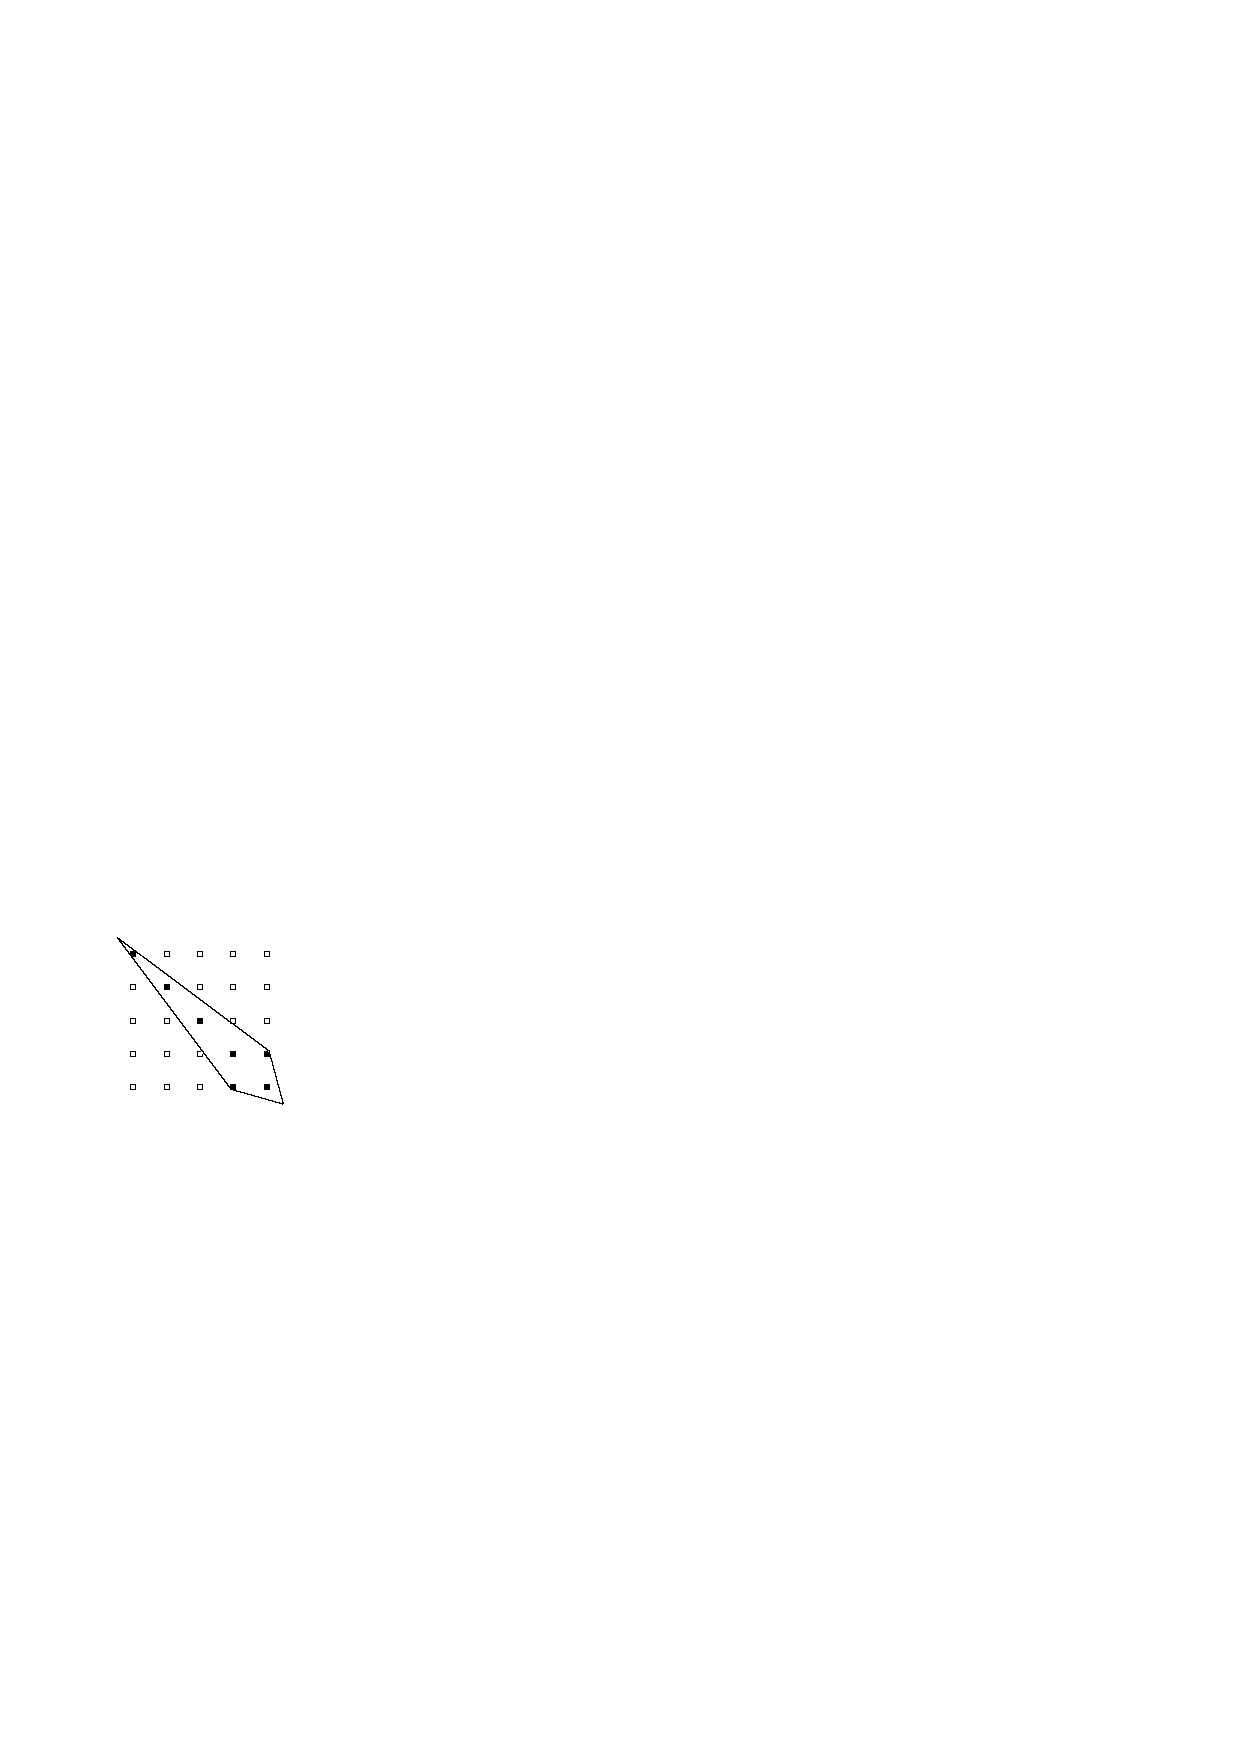
\includegraphics[scale=1.64]{pegs1}
$\quad\quad$
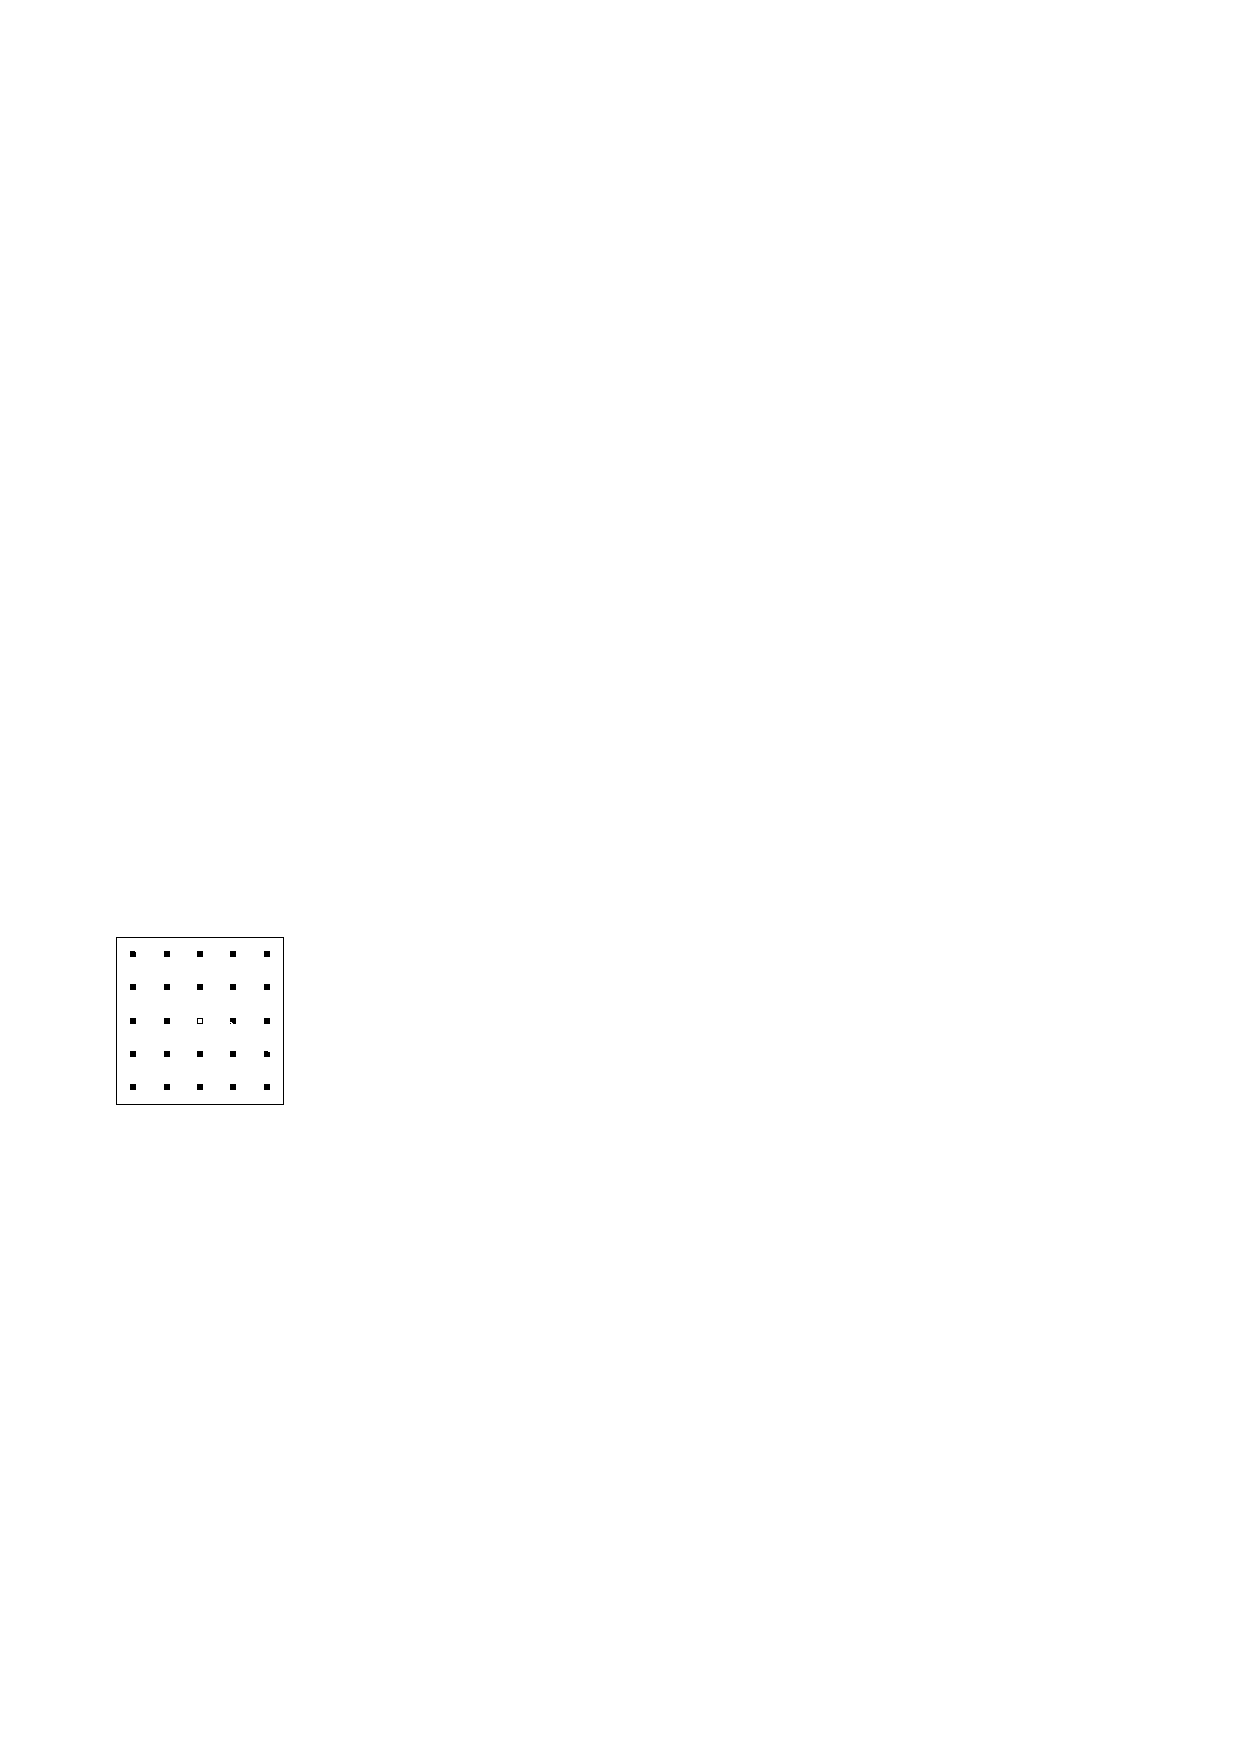
\includegraphics[scale=1.64]{pegs2}

Examples of convex polygons that achieve the values given in the output are above. In the first example Worro gets \$7, in the second he gets \$24-\$1=\$23.
